\documentclass[12pt]{extarticle}
%Some packages I commonly use.
\usepackage[portuguese]{babel}
\usepackage{graphicx}
\usepackage{framed}
\usepackage[normalem]{ulem}
\usepackage{amsmath}
\usepackage{amsthm}
\usepackage{amssymb}
\usepackage{amsfonts}
\usepackage{enumerate}
\usepackage[utf8]{inputenc}
\usepackage{float}
\usepackage{gensymb}
\usepackage[top=1 in,bottom=1in, left=1 in, right=1 in]{geometry}
\usepackage{multirow}
\usepackage{caption}
\usepackage{subcaption}
\usepackage[utf8]{inputenc}

%A bunch of definitions that make my life easier
\newcommand{\matlab}{{\sc Matlab} }
\newcommand{\cvec}[1]{{\mathbf #1}}
\newcommand{\rvec}[1]{\vec{\mathbf #1}}
\newcommand{\ihat}{\hat{\textbf{\i}}}
\newcommand{\jhat}{\hat{\textbf{\j}}}
\newcommand{\khat}{\hat{\textbf{k}}}
\newcommand{\minor}{{\rm minor}}
\newcommand{\trace}{{\rm trace}}
\newcommand{\spn}{{\rm Span}}
\newcommand{\rem}{{\rm rem}}
\newcommand{\ran}{{\rm range}}
\newcommand{\range}{{\rm range}}
\newcommand{\mdiv}{{\rm div}}
\newcommand{\proj}{{\rm proj}}
\newcommand{\R}{\mathbb{R}}
\newcommand{\N}{\mathbb{N}}
\newcommand{\Q}{\mathbb{Q}}
\newcommand{\Z}{\mathbb{Z}}
\newcommand{\<}{\langle}
\renewcommand{\>}{\rangle}
\renewcommand{\emptyset}{\varnothing}
\newcommand{\attn}[1]{\textbf{#1}}
\theoremstyle{definition}
\newtheorem{theorem}{Theorem}
\newtheorem{corollary}{Corollary}
\newtheorem*{definition}{Definition}
\newtheorem*{example}{Example}
\newtheorem*{note}{Note}
\newtheorem{exercise}{Exercise}
\newcommand{\bproof}{\bigskip {\bf Proof. }}
\newcommand{\eproof}{\hfill\qedsymbol}
\newcommand{\Disp}{\displaystyle}
\newcommand{\qe}{\hfill\(\bigtriangledown\)}
\setlength{\columnseprule}{1 pt}
\usepackage[utf8]{inputenc}

\title{Aula 8 - Introdução à Eletrostática e Lei de Coulomb}
\author{Felipe Salvador}
\date{Atualizado em \today}

\begin{document}

\maketitle

\section{Introdução}
Iniciamos os estudos sobre eletricidade falando dos fenômenos e conceitos mais básicos. Vamos enumerar diversas qualidades e definir as principais quantidades envolvidas na eletricidade. Por fim, falaremos da Lei de Coulomb, a primeira descrição precisa de força envolvendo a eletricidade.

\section{Conceitos básicos}

Nessa parte iremos discutir os conceitos fundamentais da teoria sobre eletricidade, falando sobre os principais atores e fenômenos envolvidos.
\subsection{Carga elétrica}

\textbf{A carga elétrica é uma das 3 propriedades fundamentais da matéria.} Toda matéria para ser definida, tem que ter um valor de carga elétrica associada a ela. A carga elétrica é responsável por fazer a matéria sentir uma classe de forças que chamamos de \textbf{força eletromagnética.} A principal diferença para a massa (outra propriedade fundamental) é que \textbf{a carga elétrica pode 2 sinais: positiva ou negativa.} 

Há também a possibilidade de que a carga elétrica de uma partícula seja 0, mas aí ela não sofrerá ação de uma força eletromagnética e ai não se encaixa nessa teoria.

\subsection{Fenômenos de forças de atração e repulsão de cargas}

A primeira questão que foi observada sobre as cargas era que o seu comportamento não era parecido com a gravidade. Ao invés de atrair iguais, foi observado que \textbf{cargas com sinais iguais se repelem e cargas com sinais diferentes se atraem.}
\begin{figure}[H]
    \centering
    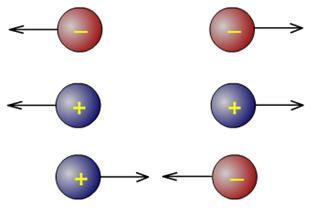
\includegraphics[width=0.4\textwidth]{cargas-eletricas.jpg}
    \caption{Diagrama de forças de atração e repulsão de cargas elétricas.}
    \label{fig:ex_1}
\end{figure}

Com isso, os fenômenos vistos na eletricidade são esses 2 somente.

\subsection{Quantização da carga elétrica}

Até o início do século 20, os cientistas acreditavam que poderiam existir cargas elétricas com qualquer valor, o que possibilitava uma variedade de estudos. Porém, com a descoberta da Mecânica Quântica e com o experimento com gotas de óleo de Millikan, houve a imposição de que as cargas elétricas tivessem o seu valor como \textbf{múltiplos inteiros de um valor base.} 

Além disso, percebeu-se que esse valor base era um valor nominal de uma partícula já conhecida na época, \textbf{o elétron}. Esse valor nominal do elétron foi descoberto pelo experimento do Millikan e é de:
\begin{equation}
    |e| \approx 1,6*10^{-19}\, C
\end{equation}
\noindent em que 'C' é uma unidade chamada de \textit{'Coulomb'} e é a unidade do Sistema Internacional para cargas elétricas.

De forma geral, qualquer carga elétrica é então:
\begin{equation}
    Q = n*|e|
\end{equation}
\noindent em que $Q$ é o valor da carga elétrica e $n$ é um número inteiro (ex: 4).

Percebeu-se que o elétron era uma carga negativa, então o $n$ é -1:
\begin{equation}
    e \approx -1,6*10^{-19}\,C
\end{equation}

\subsection{Conservação de cargas}
Um dos conceitos mais básicos e principais é que \textbf{a carga elétrica total é constante}, ou seja, somando o valor de todas as cargas elétricas num espaço, não importa o que eu faça, esse valor total sempre será o mesmo. Isso impede que só cargas positivas ou só cargas negativas sejam criadas. Só permite que eu crie um par de cargas - 1 positiva e 1 negativa.

\section{Átomos e matéria}
No século 19, diversos estudos foram feitos para entender sobre o que é constituído a matéria. Um dos primeiros resultados é a \textbf{matéria é neutra}, ou seja, há uma mesma quantidade de cargas elétricas positivas e negativas.

Os gregos antigos foram os primeiros a fazer suposições sobre a matéria. Falaram que a matéria era feita de pequenas esferas duras e indivisíveis, chamadas de \textbf{átomos}. Essa discussão foi reacesa no século 19 com Thomson, em que foi o primeiro a modelar como a matéria era composta usando cargas elétricas.  O nome desse modelo é \textbf{Pudim de Passas}: o "pudim" seria feito de uma matéria com carga positiva e as "passas" seriam os elétrons, cargas negativas.
\begin{figure}[H]
    \centering
    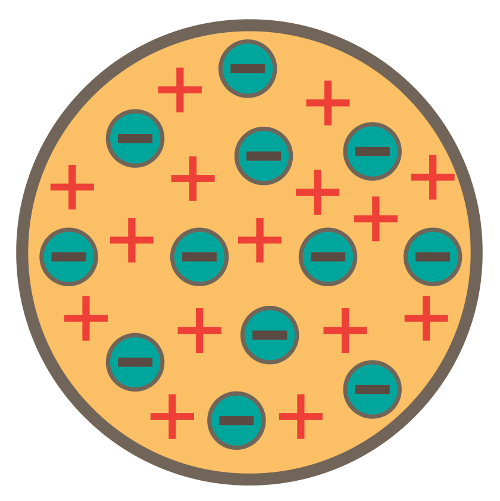
\includegraphics[width=0.4\textwidth]{representacao-dos-eletrons-fluido-positivo-no-modelo-atomico-thomson-5880b350bbb81.jpg}
    \caption{Representação do modelo atômico de Thomson}
    \label{fig:ex_2}
\end{figure}

Porém, o modelo de Thomson rapidamente foi recusado, porque ele não era capaz de descrever um experimento: O experimento de Geiger-Marsden - em que um canhão atirava partículas contra uma folha bem fina de ouro. Percebeu-se que algumas poucas partículas (1 a cada 8000) voltavam na direção do canhão, o que contradizia o modelo de Thomson.

Depois disso, Rutherford propôs um modelo se inspirando no Sistema Solar: O Sol seria o núcleo do átomo, onde estaria as cargas positivas, e os planetas orbitando em volta do Sol seriam os elétrons, as cargas negativas.
\begin{figure}[H]
    \centering
    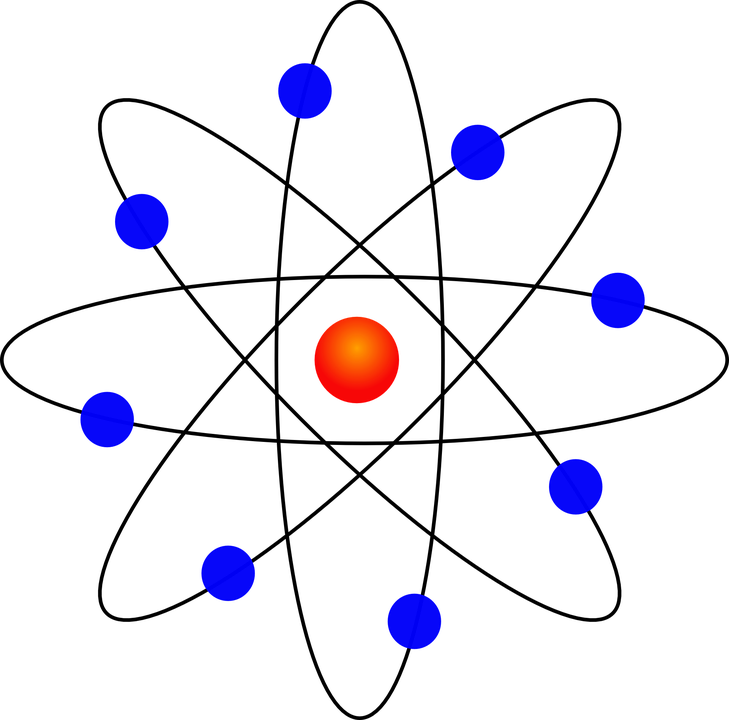
\includegraphics[width=0.4\textwidth]{b0653c823d734f39a11e617eaa929fab-467.png}
    \caption{Representação do modelo de Rutherford}
    \label{fig:ex_3}
\end{figure}

Esse modelo foi capaz de prever os resultados do experimento de Geiger-Marsden e foi aceito como um bom modelo sobre o átomo. Mais tarde, foi descoberto que o núcleo era feito por 2 partículas chamadas de \textbf{prótons e nêutrons}.
\textbf{O próton é uma partícula com carga positiva de valor: $q_p = 1,6*10^{-19}\,C$ e o nêutron é uma partícula neutra (carga igual à 0).}

Fora a carga, a primeira observação sobre o próton e o nêutron em relação ao elétron é que eles eram muito mais pesados do que o elétron. Para efeito de comparação, eles são 1836 vezes mais pesados do que o elétron.

A massa das 3 partículas e suas cargas estão na tabela abaixo:
\begin{table}[H]
    \centering
    \begin{tabular}{|c|c|c|}
         \hline
         &\textbf{Massa (kg)} & \textbf{Carga (C)}\\
         \hline
         \textbf{Próton}& $1,6*10^{-27}$ & $1,6*10^{-19}$\\
         \hline
         \textbf{Elétron}& $9,1*10^{-31}$ & $-1,6*10^{-19}$ \\
         \hline
         \textbf{Nêutron}& $1,6*10^{-27}$ & $0$ \\
         \hline
    \end{tabular}
    \caption{Tabela com os valores de massa e carga das 3 partículas que compõe a matéria}
    \label{tab:table_1}
\end{table}

Hoje, com a descoberta da mecânica quântica, os modelos de átomo envolvem outras definições, como spin, orbitais e Princípio da Exclusão de Pauli.

\section{Materiais Elétricos}
Há 2 tipos de materiais elétricos: \textbf{Condutores e Isolantes.}
\textbf{Os condutores são materiais que as cargas elétricas podem se mover com facilidade no material.} Quem se move no material são sempre os elétrons, pois eles são bem mais leves do que os núcleos dos átomos (prótons e nêutrons). Exemplos de condutores elétricos são os metais em geral.

\textbf{Os isolantes são materiais que as cargas elétricas não conseguem se mover no material por causa da ação de forças internas.} Quando tenho um material isolante, é como se os elétrons e os átomos ficassem estacionados sobre um ponto. Exemplo de isolantes elétricos é a borracha.

\section{Processos de Eletrização}
Há formas de fazer com que um objeto neutro se torne eletrizado e, logo, tenha uma carga elétrica total diferente de 0. Veremos 3 formas de fazer a eletrização:

\subsection{Eletrização por atrito}
Essa forma é quando esfregamos 2 objetos neutros feitos de materiais diferentes. Após esse processo, um objeto ficará com carga positiva, enquanto o outro objeto fica com carga negativa.
\begin{figure}[H]
    \centering
    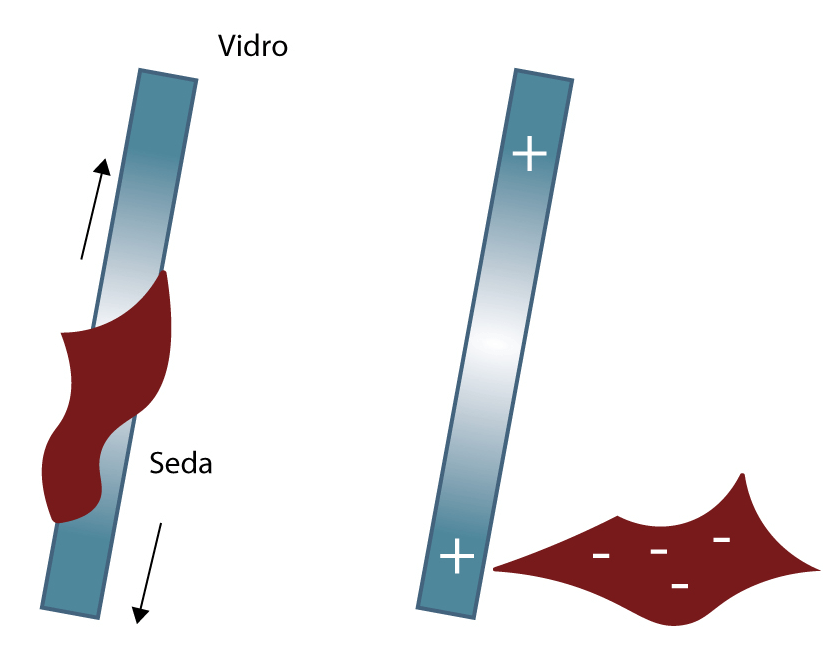
\includegraphics[width=0.4\textwidth]{eletrização-por-atrito.png}
    \caption{Exemplo de eletrização por atrito}
    \label{fig:ex_4}
\end{figure}

\subsection{Eletrização por contato}
É quando encostamos um objeto condutor com carga elétrica num outro objeto condutor, que pode ter carga elétrica.
\begin{figure}[H]
    \centering
    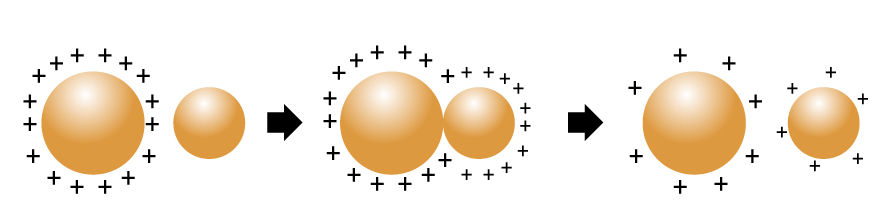
\includegraphics[width=0.4\textwidth]{eletrização-por-contato-positivamente-carregado.png}
    \caption{Exemplo de eletrização por contato}
    \label{fig:my_label}
\end{figure}

Ao final, quando separamos os 2 condutores, \textbf{os dois condutores possuem a mesma carga elétrica.}

\textit{Exemplo:} Um condutor com carga elétrica de 2 C é posto em contato com um outro condutor com carga elétrica -1 C. Qual é a carga final nos dois?

Sabemos que a carga elétrica total é conservada no processo. No início:
\begin{equation*}
    2\,C + (-1\,C) = 1\,C
\end{equation*}

Sabemos que ao final do contato, os dois tem a mesma carga: $Q\,C$, então pela conservação de carga:
\begin{equation*}
    Q + Q = 1 \implies 2Q =1 \implies Q = 0,5 \, C
\end{equation*}

\subsection{Eletrização por indução}
Essa forma de eletrização acontece quando aproximamos um condutor com carga elétrica diferente de 0 (não-nula) de um condutor neutro. O que ocorre é que o condutor eletrizado irá induzir cargas elétricas no condutor neutro, conforme a imagem a seguir:
\begin{figure}[H]
    \centering
    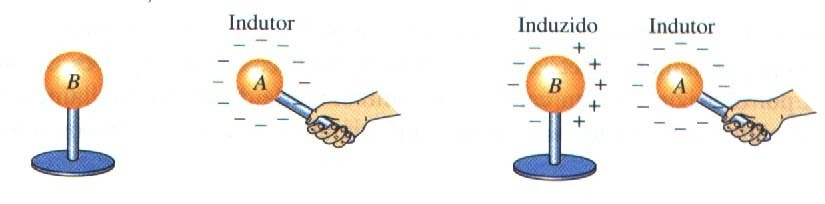
\includegraphics[width=0.7\textwidth]{eletrizacao_por_inducao.jpg}
    \caption{Descrição de como ocorre a eletrização por indução. Quando aproximamos o objeto eletrizado ao objeto neutro, será induzido cargas elétricas. As cargas elétricas de sinal oposto serão atraídas, enquanto as cargas com o mesmo sinal sofrem repulsão.}
    \label{fig:ex_5}
\end{figure}

Porém se eu ligar à uma face do objeto que tá sofrendo a indução no chão, irá ocorrer o seguinte fenômeno:
\begin{figure}[H]
    \centering
    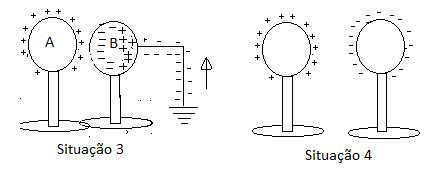
\includegraphics[width=0.7\textwidth]{indução-2.png}
    \caption{Se conectarmos o fio ao lado que está as cargas positivas (negativas), cargas negativas (positivas) subiram pelo fio para neutralizar as cargas desse lado. Quando eu desconecto o fio, o objeto induzido só sobra as cargas negativas (positivas) induzidas.}
    \label{fig:ex_6}
\end{figure}

Outros formas de eletrização por indução é quando colocamos uma objeto eletrizado dentro de um objeto inicialmente neutro: 
\begin{figure}[H]
    \centering
    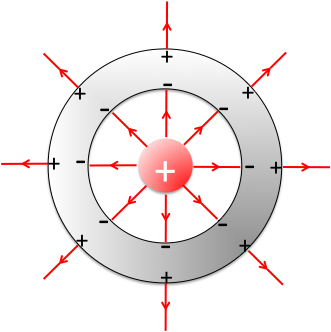
\includegraphics[width=0.3\textwidth]{qnd3i.png}
    \caption{Eletrização por indução de um objeto eletrizado posto dentro de um condutor neutro. Ele induz cargas negativas na parte de dentro, enquanto as cargas positivas são repulsadas para a parte externa.}
    \label{fig:ex_7}
\end{figure}

\section{Lei de Coulomb}
Em 1783, o físico francês Charles Coulomb escreveu uma lei empírica (a partir de experimentos) que exprime como funciona a força exercida por uma carga elétrica sobre outra carga elétrica:
\begin{equation}
    F = K_0\frac{|q_1|\,|q_2|}{d^2}
\end{equation}
\noindent em que $q_1,\,q_2$ são os valores das cargas envolvidas, $d$ é a distância entre as cargas e $K_0$ é uma constante, chamada de \textbf{constante eletrostática}. Essa constante é designada por:

\begin{equation}
    K_0 = \frac{1}{4\pi\,\varepsilon_0} = 9,0*10^9\,N.m^2.C^{-2}
\end{equation}
\noindent $\varepsilon_0$ é chamado de Permissividade Elétrica do Vácuo e tem valor: $\varepsilon_0 = 8,85*10^{-12}\,N^{-1}.m^2.C^{2}$

Importante dessa força é que ela só me dá o módulo da força. A direção da força depende dos sinais das cargas.

\begin{figure}[H]
    \centering
    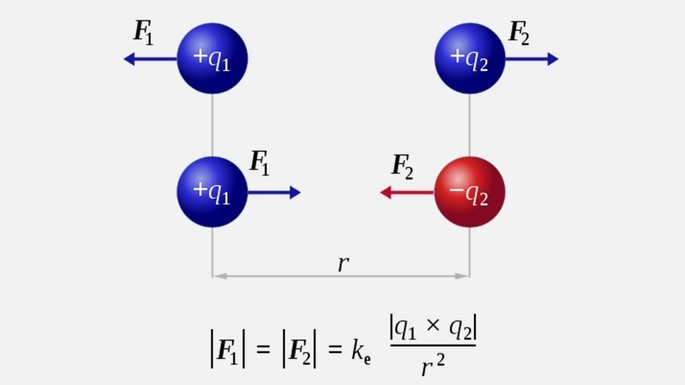
\includegraphics[width=0.6\textwidth]{atracaoerepulsaocargaseletricas-cke.jpg}
    \caption{Esquema de força descrita pela Lei de Coulomb}
    \label{fig:ex_8}
\end{figure}

\end{document}
